\chapter{Realisation}
\section{Introduction}

In this chapter, we present the working environment that allowed us to develop our application initially. Then we present the deployment diagram.

\section{Technical Environment}

The technical architecture, often also called computer architecture or software architecture, represents the overall structure of a computer system, including hardware, software, network protocols, standards used, as well as the physical and logical aspects of interactions and relationships between these different elements.

\subsection{Hardware Choices}

In this part, we mention the hardware(s) that we used to complete the work as shown in the table below (see Table \ref{tab:hardware-choices}).
\begin{table}[htbp]
    \centering
    
    \begin{tabular}{|p{2cm}|p{3cm}|p{2cm}|p{4cm}|p{2cm}|}
        \hline
        \rowcolor{purple!20} % Light green background
        Device(s) & Processor & Memory & Storage & OS \\
        \hline
        Machine & & & & \\
        Lenovo Ideapad 320  & Intel Core i3 6006u & 8 GB & 500 GB SSD and  1 TB HDD & Windows 10\\
        \hline
       \end{tabular}
       \caption{Hardware Choices}
    \label{tab:hardware-choices}
\end{table}

\subsection{Software Choices}

In this part, we detail the different tools used for configuration and development of our application.


\begin{table}[h]
    \centering
    
    \begin{tabular}{|c|c|c|}
        \hline
       \raisebox{1.3\height}{
\includegraphics[width=0.2\textwidth]{media/odoo_logo.png}} &
        
\includegraphics[width=0.2\textwidth]{media/pycharm_logo.png} &
        
\includegraphics[width=0.2\textwidth]{media/vscode.png} \\
        
        \hline
        \textbf{\cellcolor{gray!50}Odoo} & \textbf{\cellcolor{gray!50}PyCharm} & \textbf{\cellcolor{gray!50}Vscode} \\
        \hline
    \end{tabular}
    \caption{Software Used}
    \label{tab:Software Used}
\end{table}
• \textbf{Odoo} \cite{odoo}: A comprehensive suite of business applications, including CRM, e-commerce, billing, and inventory management. Odoo is highly modular and user-friendly, facilitating rapid application development and customization.

• \textbf{PyCharm} \cite{pycharm}: A Python IDE providing code analysis, debugging, unit testing, VCS integration, and Django support. PyCharm enhances productivity and code quality with its powerful features.

• \textbf{Visual Studio Code (VSCode)} \cite{vscode}: A free source-code editor for Windows, Linux, and macOS by Microsoft. It supports debugging, syntax highlighting, code completion, refactoring, and Git integration. VSCode is highly customizable with extensions.
\newpage
\subsection{Database Management System}

\begin{figure}[h]
    \centering
    
\includegraphics[width=0.5\textwidth]{media/PostgreSQL-Logo.wine.png}
    \caption{Database Management System}
    \label{fig:dbms}
\end{figure}

• \textbf{PostgreSQL}\cite{postgresql}: PostgreSQL is a powerful, open-source object-relational database management system (ORDBMS) capable of safely handling the most complex data workloads. It has several user interfaces, such as PSQL for command-line interaction and PgAdmin as a graphical administration tool.




\subsection{Programming Languages}



\begin{table}[h]
    \centering
    
    \begin{tabular}{|c|c|c|}
        \hline
        
\includegraphics[width=0.15\textwidth]{media/xml_logo.png} &
        
\includegraphics[width=0.2\textwidth]{media/python_logo.png} &
        
\includegraphics[width=0.2\textwidth]{media/css-3.png} \\
        \hline
        \textbf{\cellcolor{gray!50}XML} & \textbf{\cellcolor{gray!50}Python} & \textbf{\cellcolor{gray!50}CSS} \\
        \hline
    \end{tabular}
    \caption{Programming Languages}
    \label{tab:programming-languages}
\end{table}
\newpage

\subsection{Tools}


\begin{table}[htbp]
    \centering
   
    \begin{tabular}{|c|c|c|}
        \hline
        
\includegraphics[width=0.2\textwidth]{media/drawio.png} &
        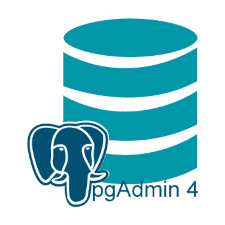
\includegraphics[width=0.2\textwidth]{media/PgAdmin4.jpg} &
        
\includegraphics[width=0.2\textwidth]{media/git.png} \\
        
        \hline
        \textbf{\cellcolor{gray!50}Drawio} & \textbf{\cellcolor{gray!50}PgAdmin4} & \textbf{\cellcolor{gray!50}git} \\
        \hline
    \end{tabular}
     \caption{Tools}
    \label{tab:Tools}
\end{table}

\begin{itemize}
    \item \textbf{Draw.io} \cite{drawio}: An online tool for creating diagrams, flowcharts, and visual representations. It is user-friendly and supports collaborative work.
    
    \item \textbf{PgAdmin 4} \cite{pgadmin}: A graphical tool for managing PostgreSQL databases, running SQL queries, and visualizing data.
    
    \item \textbf{Git} \cite{git}: A version control system for tracking code changes and managing branches. Essential for collaboration and code management.
\end{itemize}

\subsection{Platform}
\begin{table}[htbp]
    \centering
  
    \begin{tabular}{|c|}
        \hline
        
\includegraphics[width=0.2\textwidth]{media/github.png} \\
        \hline
        \textbf{\cellcolor{gray!50}GitHub \cite{github}} \\
        \hline
    \end{tabular}
      \caption{Platform}
    \label{tab:Platform}
\end{table}
\begin{itemize}
    \item \textbf{GitHub}: A web-based platform for version control and collaboration, allowing developers to manage and share their code repositories, track changes, and work on projects collaboratively with features such as pull requests, issues, and project boards.
\end{itemize}



\section*{Conclusion}
\addcontentsline{toc}{section}{Conclusion}


In this chapter, we explore the tools and technologies used in the development of the Odoo application. By leveraging \textbf{Odoo}, we facilitated the creation and customization of business applications. \textbf{PyCharm} was instrumental in enhancing our productivity with its robust Python IDE features, while \textbf{Visual Studio Code} provided a versatile and customizable coding environment. Tools such as \textbf{Drawio} for diagramming, \textbf{PgAdmin 4} for database management, and \textbf{GitHub} for version control and collaboration played a crucial role in ensuring smooth project execution and management. Together, these tools and technologies enabled the efficient and effective development of a comprehensive and modular Odoo application, \\ demonstrating the synergy of modern development practices and tools.


